The lyapunov exponent of a dynamical system is a quantity that characterizes the rate of separation of infinitesimally close trayectories\cite{Parlitz92}.\\

Suppose that we let transients decay, so that a trajectory is \emph{on} the attractor. Suppose $\mathbf{\phi}(x,t)$ is a point on the attractor at time $t$, and consider a nearby point $\mathbf{\phi}(t)+\delta(t)$ where $\delta$ is a very small separation. It can be seen in the following figure, that  $\delta(t)$ grows. The two trajectories diverge with at a rate given by

$\lVert\delta(t) \rVert \ \lVert\delta_oo \rVert e^{\lambda t}$


\begin{figure}[h]
\centering
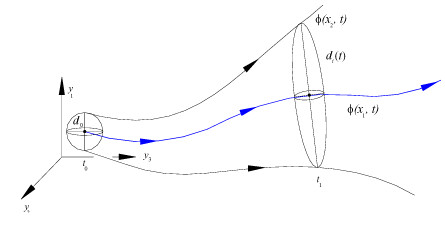
\includegraphics[scale=0.5]{imagenes/2-benford/Lyap_exp.jpg}
\caption{Neighboring trajetories separating exponentially fast with initial separation $\delta_0$ }
\end{figure}
When at least one Lyapunov exponent is positive the attractor possesses the property of sensitive dependence of initial conditions.
